\section{Lineární programování}
Úlohy lineárního programování jsou optimalisační úlohy, ve kterých je
\begin{enumerate}[(a)]
    \item cílová funkce afinní (bez újmy na obecnosti se můžeme omezit na lineární funkce)
    \item přípustná množina je konvexní polyedrická množina (tj. lze popsat pomocí konečné soustavy lineárních rovnic a
    nerovnic)
\end{enumerate}
Příklad.

Firma vyrábí 2 druhy výrobků $A$ a $B$. V tabulce je uvedeno množství materiálu (ve vhodných jednotkách) potřebný k
výrobě jednotkového množství daného druhu výrobku a také jeho prodejní cena.
\begin{center}
    \begin{tabular}{|c|c|c|l|}
        \hline
        & Materiál $X$ & Materiál $Y$ & Cena \\ \hline
        Výrobek $A$ & 2 & 3 & 6000 Kč \\ \hline
        Výrobek $B$ & 4 & 4 & 10000 Kč \\ \hline
    \end{tabular}
\end{center}
Na skladu je jen 10 jednotek materiálu $X$ a 12 jednotek materiálu $Y$. Jak mají ve firmě nastavit výrobni proces, aby
celková cena za vyrobené množství výrobků byla co největší?

Odpověď je přímo v zadání.
\begin{flalign*}
    x_1& \dots \text{množství výrobku } A& \\
    x_2& \dots \text{množství výrobku } B&
\end{flalign*}
\Opt{max}{}{6x_1 + 10x_2}{
    2x_1 + 4x_2 \: &\leq 10,\\
    3x_1 + 4x_2 \: &\leq 12,\\
    x_1, x_2 \: &\geq 0.
}

\begin{multicols}{2}
    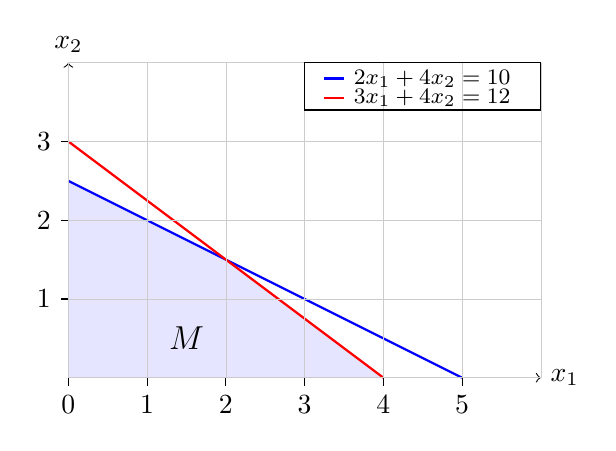
\begin{tikzpicture}[scale=1]
        \fill[blue!20,opacity=0.5]
            (0,0) --
            (0,2.5) --
            (2,1.5) -- %
            (4,0) --
            (0,0);
        \node[black] at (1.5,0.5) {\large $M$};

        \draw[->] (0,0) -- (6,0) node[right] {$x_1$};
        \draw[->] (0,0) -- (0,4) node[above] {$x_2$};

        \foreach \x in {0,1,2,3,4,5} \draw (\x,0) -- (\x,-0.1) node[below] {\x};
        \foreach \y in {1,2,3} \draw (0,\y) -- (-0.1,\y) node[left] {\y};

        % 2x1 + 4x2 = 10  => x2 = (10 - 2x1)/4
        \draw[thick,blue] (0,2.5) -- (5,0);

        % 3x1 + 4x2 = 12 => x2 = (12 - 3x1)/4
        \draw[thick,red] (4,0) -- (0,3);

        \draw[step=1cm,gray!40,very thin] (0,0) grid (6,4);

        \begin{scope}[shift={(3,3.8)}, scale=0.5]
            \draw[black] (0,0.4) rectangle (6,-0.8);
            \draw[thick,blue] (0.5,0) -- (1,0);
            \node[right] at (1,0) {\footnotesize $2x_1 + 4x_2 = 10$};

            \draw[thick,red] (0.5,-0.5) -- (1,-0.5);
            \node[right] at (1,-0.5) {\footnotesize $3x_1 + 4x_2 = 12$};
        \end{scope}
    \end{tikzpicture}

\columnbreak

    Graficky lze nalézt, že maximum se nabývá v bodě $(2, \frac{3}{2})^T$. Maximum je $f(2, \frac{3}{2}) = 27$.
\end{multicols}
Pokračování příkladu.

Obchodník chce od firmy koupit veškerý materiál ze skladu. Jaké ceny za materiál $X$ a $Y$ by měl firmě nabídnout, aby
zaplatil co nejmenší částku a firmě se přesto vyplatilo materiál prodat namísto výroby výrobků?

\newpage
Tato otázka vede na úlohu:
\begin{flalign*}
    y_1& \dots \text{cena za jednotkové množství materiálu } X& \\
    y_2& \dots \text{cena za jednotkové množství materiálu } Y&
\end{flalign*}
\Opt{min}{}{10y_1 + 12y_2}{
    2y_1 + 3y_2 \: &> 6, \\
    4y_1 + 4y_2 \: &> 10,\\
    y_1, y_2 \: &\geq 0.
}
Pozorování. Tyto dvě úlohy jsou navzájem duální.

\subsection{Zápis úlohy lineárního programování}
Je dána úloha
\Opt{min}{}{x_1 - x_2}{
    2x_1 - 3x_2 \: &= 5, \\
    -2 \leq x_2 \: &\leq 3, \\
    x_1 \: &\leq 0.
}
Zapišme úlohu v kanonickém tvaru.\\
Pomocné substituce: $y_1 = -x_1$, $x_2 = y_2 - y_3$, $y_2, y_3 \geq 0$.
\Opt{min}{}{-y_1-y_2+y_3}{
    -2y_1 - 3y_2 + 3y_3 \: &\geq 5, \\
    2y_1 + 3y_2 - 3y_3 \: &\geq -5, \\
    -y_2 + y_3 \: &\geq -3, \\
    y_2 - y_3 \: &\geq -2,\\
    y_1, y_2, y_3 \: &\geq 0.
}
Zapišme úlohu ve standardním tvaru.
\Opt{min}{}{-y_1-y_2+y_3}{
    -2y_1 - 3y_2 + 3y_3 \: &= 5, \\
    y_2 - y_3 - y_4 \: &= -2, \\
    y_2 - y_3 + y_5 \: &= 3, \\
    y_1, y_2, y_3, y_4, y_5 \: &\geq 0.
}

\subsection{Terminologie lineárního programování}
Je dána úloha
\Opt{min}{}{\langle x,c\rangle}{
    Ax \: &= b,\\
    x \: &\geq 0,
}
kde $c\in \R^n$, $b \in \R^m$ a $A \in \M_{m,n}(\R)$ splňuje
\[
    \rank A = \rank (A, b) = m \leq n.
\]
Dále se v této sekci budeme držet následujícího značení:
\begin{itemize}
    \item Přípustná množina $M = \bc{x \in \R^n \mid Ax = b, x\geq 0}$.
    \item $J(x) \coloneqq \bc{j \in \bc{1, \dots, n} \mid x_j > 0}$, kde $x = (x_1, \dots, x_n)^T \in \R^n$.
    \item $a_1, \dots, a_n \in \R^m$ sloupce matice A.
    \item Nechť $B \subseteq \bc{1, \dots, n}$ je neprázdná. Pak $A_B$ je matice tvořená sloupci matice $A$ s indexy v 
    $B$ (v daném pořadí). Je-li $x = (x_1, \dots, x_n)^T$, pak $x_B$ je sloupec tvořený prvky $x_i, i \in B$, v daném 
    pořadí.
    \item $N \coloneqq \bc{1, \dots, n} \setminus B$.
\end{itemize}

\subsection{Basický přípustný bod}\label{BPB}
Bod $x \in M$ se nazve basický přípustný bod (BPB) úlohy lineárního programování, pokud existuje $m$-prvková množina
$B \subseteq \bc{1, \dots, n}$ taková, že
\begin{enumerate}[(a)]
    \item $A_B$ je regulární,
    \item $x_j = 0$ pro každé $j \in N$.
\end{enumerate}
Množina $B$ z definice BPB se nazývá přípustná báse.

\subsection{Příklad BPB}
Nechť
$A =
    \begin{bmatrix}
        1 & 2 & 3 \\
        0 & 2 & 3
    \end{bmatrix}
$ a $b =
    \begin{bmatrix}
        5 \\
        3
    \end{bmatrix}
$. Jaké jsou BPB?
\begin{itemize}
    \item $B = \bc{1,2} \dots A_B =
    \begin{bmatrix}
        1 & 2 \\
        0 & 2
    \end{bmatrix}$. Evidentně invertibilní. \\
    $x =
    \begin{bmatrix}
    x_1 \\
    x_2 \\
    x_3
    \end{bmatrix} \dots \underbrace{Ax}_{A_B x_B +  A_N\underbrace{x_N}_{=0}}=b$. Tedy
    $\left[
        \begin{array}{cc|c}
        1 & 2 & 5 \\
        0 & 2 & 3
        \end{array}
    \right]
    \rightarrow x = \frac{1}{2}
    \begin{bmatrix}
        1 \\
        3 \\
        0
    \end{bmatrix} \in M$ je BPB.
    \item $B = \bc{1,3} \dots A_B =
    \begin{bmatrix}
        1 & 3 \\
        0 & 3
    \end{bmatrix}$. Evidentně invertibilní. \\
    Tedy
    $\left[
        \begin{array}{cc|c}
        1 & 3 & 5 \\
        0 & 3 & 3
        \end{array}
    \right]
    \rightarrow x =
    \begin{bmatrix}
        2 \\
        0 \\
        1
    \end{bmatrix} \in M$ je BPB.
    \item $B = \bc{2,3} \dots A_B =
    \begin{bmatrix}
        2 & 3 \\
        2 & 3
    \end{bmatrix}$. Evidentně není regulární. Žádný bod nemůže být BPB.
\end{itemize}

\subsection{Tvrzení o charakterisaci BPB}\label{charBPB}
Nechť $x \in M$. Pak $x$ je BPB právě tehdy, když $\bc{a_j \mid j \in J(x)}$ je lineárně nezávislá množina.

Důkaz.\\
\enquote{$\Rightarrow$}: $x$ je BPB $\implies$ existuje $B \subseteq \bc{1, \dots, n}$ $m$-prvková tak, že
$\bc{a_j \mid j \in B}$ je lineárně nezávislá. Navíc $J(x) \subseteq B$, protože $J(x)$ obsahuje ty indexy, které
odpovídají kladným komponentám a všechny komponenty indexované mimo indexy z $B$ jsou nulové.

Tedy $\bc{a_j \mid j \in J(x)}$ je lineárně nezávislá.

\enquote{$\Leftarrow$}: Je-li $|J(x) = m|$, pak jasné ($B = J(x)$).\\
Ať $|J(x)| < m$. Z předpokladu víme $\rank(A) = m$. Pak lze $J(x)$ doplnit do $m$-prvkové množiny
$B \subseteq \bc{1,\dots, n}$ tak, že $\bc{a_j \mid j \in B}$ je lineárně nezávislá. $\implies x$ je BPB. $\qed$

\subsection{Tvrzení, že dva různé BPB musí mít různé množiny \texorpdfstring{$B$}{B}} \label{ruzneBPB}
Pro každou $m$-prvkovou množinu $B \subseteq \bc{1, \dots, n}$ takovou, že $A_B$ je regulární, existuje nejvýše jedno
$x \in M$ splňující $x_j = 0$ pro každé $j \in N$.

Důkaz. Sporem.

Ať $x, y \in M$ jsou různé a splňují $x_j = y_j = 0$ pro každé $j \in N$.

\[
    \begin{rcases}
        b = Ax = \sum_{j = 1}^{n} x_j a_j = \sum_{j \in B}x_j a_j = A_B x_B \\
        b = Ay = A_B y_B
    \end{rcases} A_B x_B = A_B y_B
\]
A protože $A$ je dle předpokladu regulární, tak dostaneme:
\[
    x_B = y_B \implies x = y
\]
Což je ale spor, protože $x$ a $y$ mají být různé. $\qed$

Horní hranice počtu BPB úlohy LP je tedy $\binom{n}{m}$.

\subsection{Příklad na degenerované BPB}
Nechť
\[
    A =
    \begin{bmatrix}
    1 & 0 & 1 & 1 \\
    1 & 1 & 0 & 1
    \end{bmatrix} \quad \text{ a } \quad b =
    \begin{bmatrix}
        1 \\
        1
    \end{bmatrix}.
\]
Určete všechny basické přípustné body.

\begin{itemize}
    \item $B = \bc{1,2}$. Tedy $A_B =
        \begin{bmatrix}
            1 & 0 \\
            1 & 1
        \end{bmatrix}$ je určitě regulární.\\
        Pak očividně $\begin{bmatrix}1, 0, 0, 0\end{bmatrix}^T$ je BPB s přípustnou básí $B$.
    \item $B = \bc{1,3}$. Tedy $A_B =
        \begin{bmatrix}
            1 & 1 \\
            1 & 0
        \end{bmatrix}$ je určitě regulární.\\
        Pak $\begin{bmatrix}1, 0, 0, 0\end{bmatrix}^T$ je BPB s přípustnou básí $B$.
    \item $B = \bc{1,4}$. $A_B =
        \begin{bmatrix}
            1 & 1 \\
            1 & 1
        \end{bmatrix}$ je singulární, tedy není přípustnou básí BPB.
    \item $B = \bc{2,3}$. Tedy $A_B =
        \begin{bmatrix}
            0 & 1 \\
            1 & 0
        \end{bmatrix}$ je určitě regulární.\\
        Pak $\begin{bmatrix}0, 1, 1, 0\end{bmatrix}^T$ je BPB s přípustnou básí $B$.
    \item $B = \bc{2,4}$. Tedy $A_B =
        \begin{bmatrix}
            0 & 1 \\
            1 & 1
        \end{bmatrix}$ je určitě regulární.\\
        Pak $\begin{bmatrix}0, 0, 0, 1\end{bmatrix}^T$ je BPB s přípustnou básí $B$.
    \item $B = \bc{3,4}$. Tedy $A_B =
        \begin{bmatrix}
            1 & 1 \\
            0 & 1
        \end{bmatrix}$ je určitě regulární.\\
        Pak $\begin{bmatrix}0, 0, 0, 1\end{bmatrix}^T$ je BPB s přípustnou básí $B$.
\end{itemize}

\subsection{Příklad na souvislost BPB a krajních bodů}
Nechť
\[
    A =
    \begin{bmatrix}
    1 & 2 & 3 \\
    0 & 2 & 3
    \end{bmatrix} \quad \text{ a } \quad b =
    \begin{bmatrix}
        5 \\
        3
    \end{bmatrix}.
\]
$M = \bc{x \in \R^3_+ \mid Ax = b}$.

Již víme, že $x =
\begin{bmatrix} 
    2 \\ 0 \\ 1 
\end{bmatrix}$ a $y =
\begin{bmatrix}
    2 \\ \frac{3}{2} \\ 0
\end{bmatrix}$ jsou BPB.
\[
    Ax = b \dots
    \left[
        \begin{array}{ccc|c}
        1 & 2 & 3 & 5 \\
        0 & 2 & 3 & 3
        \end{array}
    \right] \sim
    \left[
        \begin{array}{ccc|c}
        1 & 0 & 0 & 2 \\
        0 & 2 & 3 & 3
        \end{array}
    \right]
\]
Tedy řešení soustavy $z =
\begin{bmatrix}
    2 \\ \frac{1}{2}(3-3t) \\ t
\end{bmatrix}, t \in \R$. Kdy je $z \in \R^3_+$?

Právě tehdy, když $t \geq 0$ a $1\geq t$, tedy $t \in [0,1]$.
\[
    z \in [x, y] \iff z = tx + (1-t)y =
    \begin{bmatrix}
        2 \\
        \frac{3}{2} \\
        0
    \end{bmatrix} + t
    \begin{bmatrix}
        \phantom{-}0 \\
        -\frac{3}{2} \\
        \phantom{-}1
    \end{bmatrix} =
    \begin{bmatrix}
        2 \\
        \frac{3}{2} (1-t) \\
        t
    \end{bmatrix}, t \in [0,1].
\]
Tedy $M = [x, y]$.

\subsection{Věta o souvislosti BPB a krajních bodů}
\begin{enumerate}[(a)]
    \item Nechť $x \in M$. Pak $x$ je BPB úlohy LP právě tehdy, když $x$ je krajní bod množiny $M$.
    \item $M$ je neprázdná právě tehdy, když existuje BPB úlohy LP.
\end{enumerate}

Důkaz (a).

\enquote{$\Rightarrow$}: Sporem.

Existují dva různé body $y, z \in M$ tak, že $x = \frac{y+z}{2}$. Ať $B$ je přípustná báse BPB $x$.

Pak $y_j = z_j = 0$ pro každé $j \in N$. Navíc $A_B$ je regulární dle \hyperref[BPB]{definice BPB}. Ale dle této stejné
definice platí, že $y$ a $z$ jsou BPB s přípustnou básí $B$. Ale dle \hyperref[ruzneBPB]{tvrzení} nemohou mít dva různé
BPB stejnou přípustnou bási. $\implies y = z$, což je spor.

\enquote{$\Leftarrow$}: Sporem.

Ať $x$ není BPB. Pak z \hyperref[charBPB]{charakterisace BPB} plyne, že $\bc{a_j \mid j \in J(x)}$ je lineárně závislá
množina.

$\rightarrow$ existují $d_j \in \R, j \in J(x)$, ne všechny nulové tak, že
\[
    \sum_{j\in J(x)} d_j a_j = 0.
\]
Definujme $d_j = 0$ pro každé $j \in \bc{1, \dots, n} \setminus J(x)$.

Pak $A d = 0$. Odtud $A(x\pm \alpha d) = b \pm \alpha \underbrace{A d}_{=0} = b$ pro všechna $\alpha \in \R$.

Pro dostatečně malé $\alpha > 0$ je $x \pm \alpha d \geq 0$. Pro takové $\alpha$ je $x \pm \alpha d \in M$. Pak
$x + \alpha d \not = x - \alpha d$ a navíc evidentně platí $x = \frac{(x+\alpha d) + (x - \alpha d)}{2}$. To je spor s
tvrzením, že máme krajní bod. $\qed$

Důkaz (b). Vynecháme.

\subsection{Základní věta lineárního programování}
\begin{enumerate}[(a)]
    \item Úloha LP má řešení právě tehdy, když $M$ je neprázdná a $\langle x, c\rangle$ je zdola omezená na $M$.
    \item Má-li LP řešení, pak existuje řešení úlohy LP, které je BPB.
\end{enumerate}
Důkaz (a).\\
\enquote{$\Rightarrow$}: Když máme řešení, pak určitě leží v $M$ a je určitě zdola omezená, protože to je právě to ono
řešení.

\enquote{$\Leftarrow$}: \href{https://cs.wikipedia.org/wiki/Weierstrassova_v%C4%9Bta}{Weierstrassova věta}. $\qed$

Důkaz (b). \\ Ať $\hat x \in \argmax_{x \in M} \langle x,c\rangle$. \\
Protože $M$ je kompaktní a konvexní, tak víme $\hat x \in \conv(\ext(M))$.

$\ext(M) \dots$ konečná množina, tj. $\ext(M) = \bc{e_1, \dots, e_k}$.
\[
    \underset{\text{obal}}{\overset{\text{konvexní}}{\implies}} \hat x = \sum_{i=1}^{l} \lambda_i e_i \text{ pro nějaké }
    \lambda_1, \dots, \lambda_l \geq 0 \text{ a } \sum \lambda_i = 1.
\]
Alespoň jeden krajní bod musí být mezi $e_i$. 
Ať $e_N \in \ext(M)$ splňuje $\langle e_N, c\rangle = \min_{i \in \bc{1, \dots, l}} \langle e_i, c\rangle$.

\[
    \langle \hat x, c\rangle = \sum_{i=1}^{l} \lambda_i \langle e_i, c\rangle \geq \left(\sum_{i=1}^{l} \lambda_i\right)
    \langle e_N, c\rangle = \langle e_N, c\rangle \implies e_N \in \argmax_{x \in M} \langle x, c\rangle. \qed
\]

\subsection{Příklad na hledání duální úlohy}
Mějme úlohu
\Opt{min}{}{x_1 + 2x_2}{
    x_1 + x_2 \: &\geq 1 \dots -x_1 -x_2 + 1 \leq 0, \\
    x_1, x_2 \: &\geq 0.
}
\begin{enumerate}[(a)]
    \item Najděte duální úlohu, jestliže $x_1, x_2 \geq 0$ je přímé omezení.
    \item Najděte duální úlohu, jestliže $x_1, x_2 \in \R$ je přímé omezení.
\end{enumerate}
(a) $L(x_1, x_2, \mu) = x_1 + 2x_2 + \mu(-x_1 -x_2 + 1)$
\[
    \varphi(\mu) = \inf_{(x_1, x_2) \in \R_+^2} L(x_1, x_2, \mu) = \inf_{(x_1, x_2) \in \R_+^2} (1-\mu)x_1 + 
    (2-\mu)x_2 + \mu
\]
\[
    \varphi(\mu) = \underbrace{\left[\inf_{x_1 \in \R_+} (1-\mu)x_1\right]}_{=
    \begin{cases}
        0 &\text{ pro } 1 \geq \mu, \\
        - \infty &\text{ pro } 1 < \mu.
    \end{cases}} + \underbrace{\left[\inf_{x_2 \in \R_+} (2-\mu)x_2\right]}_{=
    \begin{cases}
        0 &\text{ pro } 2 \geq \mu, \\
        - \infty &\text{ pro } 2 < \mu.
    \end{cases}} + \mu
\]
\[
    \implies \varphi(\mu) =
    \begin{cases}
        \mu &\text{ pro } \mu \in [0,1], \\
        -\infty &\text{ pro } \mu \not\in [0,1].
    \end{cases}
\]
A tedy duální úloha je
\Opt{max}{}{\mu}{
    \mu &\in [0,1].
}

(b) $L(x_1, x_2, \mu_1, \mu_2, \mu_3) = x_1 + 2x_2 + \mu_1(-x_1 -x_2 + 1) + \mu_2(-x_1) + \mu_3(-x_2)$
\[
    \varphi(\mu) = \inf_{(x_1, x_2) \in \R^2} L(x_1, x_2, \mu_1, \mu_2, \mu_3) = \inf_{(x_1, x_2) \in \R^2} 
    (1-\mu_1 - \mu_2)x_1 + (2-\mu_1-\mu_3)x_2 + \mu_1
\]
\[
    \varphi(\mu) = \underbrace{\left[\inf_{x_1 \in \R}(1-\mu_1-\mu_2)x_1\right]}_{=
    \begin{cases}
        0 & \text{ pro } 1-\mu_1-\mu_2 = 0, \\
        -\infty & \text{ pro } 1-\mu_1-\mu_2 \not= 0.
    \end{cases}} + \underbrace{\left[\inf_{x_2 \in \R}(2 - \mu_1 - \mu_3)x_2\right]}_{
    \begin{cases}
        0 & \text{ pro } 2-\mu_1-\mu_3 = 0, \\
        -\infty & \text{ pro } 2-\mu_1-\mu_3 \not= 0.
    \end{cases}} + \mu_1
\]
\[
    \varphi(\mu_1, \mu_2, \mu_3) = 
    \begin{cases}
        \mu_1 &\text{ pro } D_\varphi = \bc{(\mu_1, \mu_2, \mu_3) \in \R^3_+ \quad \middle| \quad 1-\mu_1-\mu_2 = 0, 
         2-\mu_1-\mu_3 = 0}, \\
        - \infty & \text{ jinak.}
    \end{cases}
\]
A tedy duální úloha je
\Opt{max}{}{\mu_1}{
    1 - \mu_1 - \mu_2 \: &= 0, \\
    2 - \mu_1 - \mu_3 \: &= 0, \\
    \mu_1, \mu_2, \mu_3 \: &\geq 0.
}

\subsection{Tvrzení o množině všech řešení úlohy LP}
Množina všech řešení úlohy LP je konvexní polyedrická množina.

\subsection{Příkad na Simplexovu metodu}
Je dána úloha
\Opt{min}{}{-x_1 - 3x_2}{
    2x_1 + 3x_2 + x_3 \: &= 6, \\
    -x_1 + x_2 + x_4 \: &= 1, \\
    x_1, x_2, x_3, x_4 \: &\geq 0.
}

\begin{equation*}
    \begin{array}{c}
        \\
        z \\
        x_3 \\
        x_4 \\
    \end{array}
    \begin{bmatrix}
        \begin{array}{cccc|c}
            x_1 & x_2 & x_3 & x_4 & b \\ \hline
            -1 & -3 & 0 & 0 & 0 \\ \hline
            \phantom{-}2 & \phantom{-}3 & 1 & 0 & 6  \\
            -1 & \phantom{-}1 & 0 & 1 & 1
        \end{array}
    \end{bmatrix}
    \text{; BPB je }
    \begin{bmatrix}
        0 \\
        0 \\
        6 \\
        1
    \end{bmatrix}.
\end{equation*}
Vyměníme $x_2$ a $x_4$ v BPB.\\
$x_2 = 1 + x_1 - x_4$\\
$\rightarrow z = -x_1 - 3(1+x_1-x_4) = -4x_1 + 3x_4 - 3$\\
$\rightarrow x_3 = 6 - 2x_1 - 3(1+x_1-x_4) = 3-5x_1+3x_4$

\begin{equation*}
    \begin{array}{c}
        \\
        z \\
        x_3 \\
        x_2 \\
    \end{array}
    \begin{bmatrix}
        \begin{array}{cccc|c}
            x_1 & x_2 & x_3 & x_4 & b \\ \hline
            -4 & 0 & 0 & \phantom{-}3 & -3 \\ \hline
            -5 & 0 & 0 & \phantom{-}3 & \phantom{-}3  \\
            \phantom{-}1 & 0 & 0 & -1 & \phantom{-}1
        \end{array}
    \end{bmatrix}
    \text{; BPB je }
    \begin{bmatrix}
        0 \\
        1 \\
        3 \\
        0
    \end{bmatrix}.
\end{equation*}
% TODO: dodělat

\subsection{Tvrzení o vztahu přípustné množiny a hodnoty cílové funkce}
Přípustná množina $M$ úlohy LP je neprázdná právě tehdy, když v bodě minima 
$\begin{bmatrix} \hat x \\ \hat y \end{bmatrix} \in \Omega$ úlohy $F_1$ tak, že $g(\hat x, \hat y) = 0$.
V tomto případě je $\hat y = 0$.

Důkaz.

\enquote{$\Rightarrow$}: Ať $\hat x \in M$. Pak $v = \begin{bmatrix} \hat x \\ 0 \end{bmatrix}$ leží v $\Omega$ a 
$g(v) = 0$ (tj. $v$ je řešení úlohy $(F_1)$ splňující $g(v) = 0$). A to jsme přesně chtěli dokázat. $\qed$

\enquote{$\Leftarrow$}: Ať $\begin{bmatrix} \hat x \\ \hat y \end{bmatrix}$ je řešení úlohy ($F_1$), splňující 
$g(\hat x, \hat y) = 0$. Pak $\hat y = 0$, a tedy $b = A \hat x + \hat y = A \hat x$. \\ A protože $\hat x \geq 0$, tak 
$\hat x \in M$. $\qed$

\subsection{Příklad dvoufázové Simplexové metody}
Je dána úloha
\Opt{min}{}{x_2}{
    x_1 \: &= 1, \\
    x_1 - x_2 \: &= 2, \\
    x_1, x_2 \: &\geq 0.
}
Sloupeček pravých stran je větší roven nule, takže můžeme použít dvoufázovou Simplexovu metodu.

1. fáze:
\Opt{min}{}{y_1 + y_2}{
    x_1 + y_1 \: &= 1, \\
    x_1 - x_2 + y_2 \: &= 2, \\
    x_1, x_2, y_1, y_2 \: &\geq 0.
}
% TODO: dodělat a vyřešit situaci s optAs - přednáška 10

\subsection{Tvrzení o primární a duální úloze}
Nechť $A \in \M_{m,n}(\R)$, $c \in \R^n$ a $b \in \R^m$. Duální úloha k úloze
\[
    \left.
    % \Opt{min}{}{\langle x, c \rangle}{
    %     Ax \: &\geq b, \\
    %     x \: &\geq 0.
    % }
    \begin{aligned}
        &\text{minimalizujte}&& \langle x, c \rangle \\
        &\text{za podmínky}  && Ax \geq b, \\
        &                    && x \geq 0.
    \end{aligned}
    \right\} (P)
\]
je
\[
    \left.\begin{aligned}
        &\text{maximalisujte}&& \langle y,b \rangle \\
        &\text{za podmínky}  && A^Ty \geq c, \\
        &                    && y \geq 0.
    \end{aligned}
    \right\} (D)
\]
Důkaz. 
\[
    L(x, y) = \langle x, c\rangle + \langle y, b- Ax\rangle = \langle x, c\rangle + \langle y, b\rangle - 
    \underbrace{\langle y, Ax\rangle}_{\langle A^Ty, x\rangle} = \langle x, c-A^Ty\rangle + \langle y, b\rangle
\]
\[
    \inf_{x\geq 0} L(x, y) = \langle y, b\rangle + \inf_{x\geq 0} \langle x, c-A^Ty\rangle =
    \begin{cases}
        \langle y, b\rangle & \text{je-li } c-A^Ty \geq 0, \\
        - \infty & \text{jinak.}
    \end{cases}
\]
Tedy duální úloha k $(P)$ je
\Opt{max}{}{\langle y,b \rangle}{
    c-A^T y \: &\geq 0, \rightarrow A^T y \leq c \\
    y \: &\geq 0. \qed
}

\subsection{Hledání duální úlohy k duální úloze}
Mějme
\[
    \left.\begin{aligned}
        &\text{maximalisujte}&& \langle y,b \rangle \\
        &\text{za podmínky}  && A^Ty \geq c, \\
        &                    && y \geq 0.
    \end{aligned}
    \right\} (D)
\]
Přepíšeme:
\[
    \begin{array}{r@{\quad}l@{\qquad}c@{\qquad}r@{\quad}l}
    \text{minimalisujte}& -\langle y, b \rangle&           &\text{minimalisujte}& \langle y, -b \rangle \\
    \text{za podmínky}  & A^T y \leq c,        & \text{tj.}&\text{za podmínky}  & (-A^T) y \geq -c, \\
                        & y \geq 0.            &           &                    & y \geq 0.
    \end{array}
\]
Duální úloha po tom je:
\[
    \begin{array}{r@{\quad}l@{\qquad}c@{\qquad}r@{\quad}l}
        \text{maximalisujte}& \langle x,-c \rangle&           & \text{minimalisujte}& \langle x,c \rangle \\
        \text{za podmínky}  &(A^T)^Tx \leq -b,    & \text{tj.}&\text{za podmínky}   & Ax \geq b, \\
                            & x \geq 0.           &           &                     & x \geq 0.
    \end{array}
\]

\subsection{Věta o silné dualitě pro LP}
Úloha $(P)$ má řešení právě tehdy, když má řešení úloha $(D)$. V takovém případě jsou hodnoty obou úloh stejné.

Nechť $\hat f < \infty$ a cílová funkce $f : \R^n \rightarrow \R$ je konvexní. Předpokládejme, že platí alespoň jedna z 
následujících podmínek
\begin{enumerate}[(a)]
    \item Komponenty $g_1, \dots, g_k$ zobrazení $g$ splňují \hyperref[slaterPodm]{Slaterovu podmínku} regularity.
    \item Zobrazení $g$ je \hyperref[sec:afin]{afinní} a $\Omega$ je konvexní polyedrická množina.  
\end{enumerate}
Potom $\hat f = \hat \varphi$. Je-li navíc $\hat f \in \R$, pak existuje řešení úlohy $(D)$.

Důkaz vynecháme.

\subsection{Simplexová metoda a řešení duální úlohy}\label{simplDual}
Do úlohy $(P)$ zaveďme doplňkové proměnné $y = (y_1, \dots, y_m)^T$. Tím dostaneme úlohu
\[
    \left.\begin{aligned}
        &\text{minimalizujte}&& \langle x, c \rangle \\
        &\text{za podmínky}  && Ax -y \geq b, \\
        &                    && x,y \geq 0.
    \end{aligned}
    \right\} (\widetilde{P})
\]
Je-li výsledná simplexová tabulka
\[
    \begin{array}{cccc cc|c}
        \widetilde{c}_1 & \cdots & \widetilde{c}_n & \widetilde{c}_{n+1} & \cdots & \widetilde{c}_{n+m} & \cdots \\ \hline
        \vdots      & \cdots & \vdots      & \vdots          & \cdots & \vdots          & \vdots \\
    \end{array}
\]
kde $\widetilde{c_1}, \dots, \widetilde{c}_{m+n} \geq 0$ a sloupce na lévé straně odpovídají postupně proměnným 
$x_1, \dots, x_n, y_1, \dots, y_m$. Pak $\hat y = \left(\widetilde{c}_{n+1},\dots, \widetilde{c}_{m+n}\right)^T$ je řešením 
úlohy $(D)$.

\subsection{Příklad řešení duální úlohy}
Je dána dvojice vzájemně duálních úloh
\[
    \begin{array}{r@{\quad}l@{\qquad}c@{\qquad}r@{\quad}l}
        \text{minimalisujte}& \langle x,c \rangle&           & \text{maximalisujte}& \langle y,b \rangle \\
        \text{za podmínky}  & Ax \geq b,         & \text{tj.}&\text{za podmínky}   & A^Ty \leq c, \\
                            & x \geq 0.          &           &                     & y \geq 0.
    \end{array}
\]
kde $A = 
\begin{bmatrix}
    0 & 4 & 1 \\
    1 & 1 & 0
\end{bmatrix}$, $b = 
\begin{bmatrix}
    2 \\ 1
\end{bmatrix}$, $c = 
\begin{bmatrix}
    1 \\ 2 \\ 4
\end{bmatrix}$.

Zaměřme se na primární úlohu.
Tedy doplníme doplňkové proměnné dle \hyperref[simplDual]{předchozí poznámky}.
\optAs{min}{\left\langle 
\begin{bmatrix}
    x_1 \\ x_2 \\ x_3
\end{bmatrix}, 
\begin{bmatrix}
    1 \\ 2 \\ 4
\end{bmatrix}\right\rangle}{%
\begin{bmatrix}
    0 & 4 & 1 & -1 & \phantom{-}0 \\
    1 & 1 & 0 & \phantom{-}0 & -1
\end{bmatrix}
\begin{bmatrix}
    x_1 \\ x_2 \\ x_3 \\ y_1 \\ y_2
\end{bmatrix} \geq 
\begin{bmatrix}
    2 \\ 1
\end{bmatrix} \\
x_1, \dots, y_2 \geq 0
}
Simplexová tabulka:
\[
    \begin{array}{c ccccc|c}
           &x_1 & x_2 & x_3 & y_1 & y_2 &  \\
           & 1 & 2 & 4 & 0 & 0 & 0 \\ \hline
        x_3& 0 & 4 & 1 &-1 & 0 & 2 \\
        x_1& 1 & 1 & 0 & 0 &-1 & 1 \\
           & 0 &-15& 0 & 4 & 1 & -9\\ \hline
        x_3& 0 & 4 & 1 &-1 & 0 & 2 \\
        x_1& 1 & 1 & 0 & 0 &-1 & 1
    \end{array}
\]
Zafixujme si sloupec $x_2$, protože má v sobě záporný koeficient. Teď vhodně vybrat řádek $\rightarrow$ vezmeme pravou 
stranou a podělíme ji koeficientem, tedy $\frac{2}{4}=\frac{1}{2}$ a $\frac{1}{1}=1$. Vybereme menší podíl.
\[
{   
    \renewcommand{\arraystretch}{1.25}
    \begin{array}{c ccccc|c}
           &x_1 & x_2 & x_3 & y_1 & y_2 &  \\
           & 0 & 0 & \phantom{-}\frac{15}{4} & \phantom{-}\frac{1}{4} & \phantom{-}1 & -9 + \frac{15}{2}\\ \hline
        x_2& 0 & 1 & \phantom{-}\frac{1}{4} &-\frac{1}{4} & \phantom{-}0 & \frac{1}{2} \\
        x_1& 1 & 0 & -\frac{1}{4} & \phantom{-}\frac{1}{4} &-1 & \frac{1}{2} \\
    \end{array}
}
\]
Protože v levé části prvního řádku není žádný záporný koeficient, algoritmus končí.

Úloha má řešení $\left(\frac{1}{2}, \frac{1}{2}, 0, 0, 0 \right)^T$. Tedy řešení původní primární úlohy je 
$\left(\frac{1}{2}, \frac{1}{2}, 0\right)^T$. A když dosadíme, tak zjistíme, že toto je řešení i duální úlohy.

\subsection{Hledání duální úlohy}
V $\R^n$ jsou daný množiny bodů $A = \bc{a_1, \dots, a_k}$ a $B = \bc{b_1, \dots, b_l}$. Ať $w \in \R^n$ a 
$\lambda \in \R$. K úloze
\optAs{min}{h(w,\lambda) = \frac{1}{2}\| w\|^2}{%
    \langle a_i, w\rangle + \lambda \geq 1 & \text{ pro všechna } i = 1, \dots, k, \\
    \langle b_j, w\rangle + \lambda \leq -1 & \text{ pro všechna } j = 1, \dots, l.
}
Zkonstruujte úlohu duální (přímé omezení je $w \in \R^n$, $\lambda \in \R$).
\[
    L(w, \lambda, y, z) = \frac{1}{2} \sum_{i=1}^{k}y_i \left[1-\langle a_i, w\rangle - \lambda\right] +
    \sum_{j=1}^{l}z_j \left[1+ \langle b_j, w\rangle + \lambda\right]
\]
\[
    \inf_{w \in \R^n, \lambda \in \R} L(w, \lambda, y, z) = ?
\]
Pro fixní $y \in \R^k, z \in \R^l$ je $(w, \lambda) \mapsto L(w, \lambda, y, z)$ konvexní funkce.
\[
    \underbrace{\nabla_w L(w, \lambda, y, z)}_{= \begin{bmatrix} \partial w_1 L \\ \vdots \\ \partial w_u L\end{bmatrix}} 
    = w - \sum_{i=1}^{k}a_iy_i + \sum_{i=1}^{l}b_i z_i = 0
\]
\[
    \implies w = \sum_{i=1}^{k} a_i y_i - \sum_{i=1}^{l}b_i z_i \implies \sum_{i=1}^{k}y_i = \sum_{i=1}^{l}z_i
\]
A tedy máme:
\begin{align}
    \varphi(y, z) = \frac{1}{2} \left\langle \sum_{i=1}^{k}a_i y_i - \sum_{i=1}^{l}b_i z_i, 
    \sum_{j=1}^{k}a_j y_j - \sum_{j=1}^{l}b_j z_j \right\rangle
    + \sum_{i=1}^{k}y_i + \sum_{i=1}^{l}z_i  \\ - \sum_{i=1}^{k}y_i \left\langle a_i, \sum_{j=1}^{k}a_j y_j
    - \sum_{j=1}^{l}b_jk_j\right\rangle + \sum_{i=1}^{l}z_i \left\langle b_i, \sum_{j=1}^{k}a_j y_i 
    - \sum_{j=1}^{l}b_j z_j\right\rangle
\end{align}
Což upravíme:
\begin{align}
    \varphi(y, z) &= \frac{1}{2} \left[
       \sum_{i=1}^{k} \sum_{j=1}^{l} z_i y_j \langle a_i, a_j \rangle
     - \sum_{i=1}^{k} \sum_{j=1}^{l} y_i z_j \langle a_i, b_j \rangle
     - \sum_{i=1}^{l} \sum_{j=1}^{k} z_i y_j \langle b_i, a_j \rangle
     + \sum_{i=1}^{k} \sum_{j=1}^{l} z_i y_j \langle b_i, b_j \rangle
    \right] \\
    &+ \sum_{i=1}^{k} y_i + \sum_{i=1}^{l} z_i
     - \sum_{i=1}^{k} \sum_{j=1}^{k} y_i y_j \langle a_i, a_j \rangle
     + \sum_{i=1}^{k} \sum_{j=1}^{l} y_i y_j \langle a_i, b_j \rangle \\
    &+ \sum_{i=1}^{k} \sum_{j=1}^{l} z_i y_j \langle b_j, a_j \rangle
     - \sum_{i=1}^{l} \sum_{j=1}^{l} z_i z_j \langle b_i, b_j \rangle
\end{align}
\begin{multicols}{2}
    A tedy:
    \begin{align}
        \varphi(y, z) &= -\frac{1}{2}\sum_{i=1}^{k}\sum_{j=1}^{k}y_i y_j \langle a_i, a_j\rangle \\
        &+ \sum_{i=1}^{k}\sum_{j=1}^{l}y_i z_j \langle a_i, b_j\rangle \\
        &- \frac{1}{2}\sum_{i=1}^{l}\sum_{j=1}^{l}y_i z_j \langle b_i, b_j\rangle \\
        &+ \sum_{i=1}^{k}y_i + \sum_{i=1}^{l}z_i
    \end{align}
    
    Hledaná duální úloha je:
    \begin{align*}
        \text{maximalisujte } \varphi(y, z) \\
        \text{za podmínek } \sum_{i=1}^{k}y_i - \sum_{j=1}^{l}z_j = 0& \\
        y, z \geq 0& 
    \end{align*}
\end{multicols}
